\newcommand{\arcsinh}{\mathrm{arcsinh}}

    \problem
    \begin{question}
        Let us revisit the following SDE with general drift and volatility
        \begin{equation}\label{generalSDE}
        \left\{
        \begin{array}{ll}
        dX_t=a(t,X_t)dt+b(t,X_t)dW_t,& t\geq0,\\
        X_0=x_0, x_0\in\mathbb R,
        \end{array}
        \right.
        \end{equation}
        where $a$ and $b$ are continuous functions which are uniformly Lipschitz continuous in $x$ with Lipschitz coefficient $K$ as described in class.  Prove that (\ref{generalSDE}) exists at least one solution $X_t$ by the successive approximation approach.
    \end{question}
    \begin{proof}
        Consider the solution in a given interval $[0,T]$.
        For any fixed but arbitrary $\omega\in\Omega$,
        we construct $X_t^{(n)}$ as follows,
        \begin{equation}
            \label{eq:induction formula}
            X_t^{(n+1)}=x_0+\int_0^ta(s,X_s^{(n)})\diff s
            +\int_0^tb(s,X_s^{(n)})\diff W_s,
            \ X_t^{(0)}=x_0
        \end{equation}
        And we claim that for any $t\in[0,T]$,
        \[\left|X_t^{(n+1)}-X_t^{(n)}\right|
        \leq x_0\frac{K^n}{n!}(t+W_t)^{n}\]
        To see this\marginnote{I have to say the proof about the claim
        is not correct -- or even the claim is not.
        Actually you can find that I did a bad job when handling
        $(t+W_t)^n$ and $|t+W_t|^n$ (I exchanged them to access my goal).

        I guess my claim holds true
        at least for a subsequence (I tried but failed), in this way the subsequence
        is Cauchy, and we still can prove the existence of the solution.
        },
        we argue by mathematical induction.
        It is easy to see that the base case $n=0$ holds true.
        Assume the induction hypothesis that for a particular
        $k$, case $n=k-1$ holds, i.e.,
        \[\left|X_t^{(k)}-X_t^{(k-1)}\right|
        \leq x_0\frac{K^{k-1}}{(k-1)!}|t+W_t|^{k-1}\]
        It follows that
        \[\begin{aligned}
            &\left|X_t^{(k+1)}-X_t^{(k)}\right|\\
            =&\left|\int_0^t\left(a(s,X_s^{(k)})-a(s,X_s^{(k-1)})\right)\diff s
            +\int_0^t\left(b(s,X_s^{(k)})-b(s,X_s^{(k-1)})\right)\diff W_s\right|\\
            \leq&K\int_0^t\left|X_s^{(k)}-X_s^{(k-1)}\right|(\diff s+\diff W_s)\\
            \leq&x_0\frac{K^k}{(k-1)!}\int_0^t(s+W_s)^{k-1}(\diff s+\diff W_s)
        \end{aligned}\]
        And we have from It\^o's lemma that
        \[\diff\left(\frac{(t+W_t)^{n+1}}{n+1}\right)
        =(t+W_t)^n\diff W_t+(t+W_t)^n\diff t+\frac{1}{2}n(t+W_t)^{n-1}\diff W_t\]
        i.e.,
        \[(t+W_t)^n(\diff t+\diff W_t)
        =\frac{\diff\left((t+W_t)^{n+1}\right)}{n+1}
        -\frac{n}{2}(t+W_t)^{n-1}\diff W_t\]
        Hence
        \[\left|X_t^{(k+1)}-X_t^{(k)}\right|\leq
        x_0\frac{K^k}{(k-1)!}\int_0^t(s+W_s)^{n-1}(\diff s+\diff W_s)
        \leq\frac{K^k}{k!}|t+W_t|^{k+1}\]
        that is, the statement about case $n=k$ also holds true,
        establishing the inductive step. So our claim follows by
        mathematical induction.

        Therefore,
        \[\sup_{t\in[0,T]}
        \left|X_t^{(n+1)}-X_t^{(n)}\right|
        \leq\frac{x_0M(T)^n}{n!}\]
        where $M(T)=K\max_{t\in[0,T]}|t+W_t|$.
        Then for any $n<m$,
        \[\sup_{t\in[0,T]}\left|X_t^{(n)}-X_t^{(m)}\right|
        \leq x_0\sum_{i=n}^\infty\frac{M(T)^i}{i!}
        \to 0\quad (n\to\infty)\]
        It follows that $X_t^{(n)}$ is Cauchy,
        thus there exists some $X_t$ s.t.
        $X_t^{(n)}\to X_t$
        uniformly as $n\to\infty$.
        And it is easy to see that $X_t$ is the solution
        if we send $n\to\infty$ on BHS of \cref{eq:induction formula}.
    \end{proof}

    \problem
    \begin{question}
        Let $X_t$ satisfy the SDE
        \[dX_t=f(t,X_t)dt+g(t)X_tdW_t,\]
        $f$ and $g$ being continuous deterministic functions.  Verify that the integrating factor
        \[I(t)=e^{-\int_0^t g(s)dW_s+\frac{1}{2}\int_0^tg^2(s)ds},\]
        satisfies
        \[d(I_tX_t)=I_tf(t,X_t).\]
        Remark: In order to understand the integrating factor of SDE, it is better that you understand that of the ODE first (and also how to derive this integrating factor as we have illustrated in class).  Then in light of this identity, $Y_t=I_tX_t$ satisfies
        \[dY_t=I_tf(t,Y_t/I_t)dt\]
        which (might) can be solved by the methods we know.  It seems necessary to mention that, sometimes there are several methods that one can solve a SDE and sometimes not, therefore it is necessary for you to know how to tackle one problem from different approaches in order to better understandings.
    \end{question}
    Denote
    \[A_t:=-\int_0^tg(s)\diff W_s+\frac{1}{2}\int_0^tg^2(s)\diff s\]
    then $A_t$ is an It\^o process as
    \[\diff A_t=-g(t)\diff W_t+\frac{1}{2}g^2(t)\diff t\]
    hence
    \[\begin{aligned}
        \diff I_t&=\diff \e^{A_t}\\
        &=\e^{A_t}\left(\diff A_t+\frac{1}{2}(\diff A_t)^2\right)\\
        &=\e^{A_t}(-g(t)\diff W_t+g^2(t)\diff t)\\
        &=I_t(-g(t)\diff W_t+g^2(t)\diff t)
    \end{aligned}\]
    It follows that
    \[\diff I_t\diff X_t=-\e^{A_t}g^2(t)X_t\diff t=-I_tX_tg^2(t)\diff t\]
    therefore,
    \[\begin{aligned}
        &\diff(I_tX_t)\\
        =&I_t\diff X_t+X_t\diff I_t+\diff I_t\diff X_t\\
        =&I_tf(t,X_t)\diff t+I_tg(t)\diff W_t+I_tX_t(-g(t)\diff W_t+g^2(t)\diff t)
        -I_tX_tg^2(t)\diff t\\
        =&I_tf(t,X_t)\diff t
    \end{aligned}\]

    \problem
    \begin{question}
        Solve the following SDEs by the method of integrating factors
        \begin{enumerate}[label=(\alph*)]
        \item $dX_t=\alpha X_tdW_t$;
        \item $dX_t=rdt+\alpha X_tdW_t$;
        \item $dX_t=X_tdt+\alpha X_tdW_t$;
        \item $dX_t=\frac{1}{X_t}dt+\alpha X_tdW_t$, $X_0>0$.
        \end{enumerate}
    \end{question}
    \begin{subproblem}[(\alph*)]
        \item
        We have that
        \[f(t,X_t)=0,g(t)=\alpha\]
        thus
        \[I_t=\e^{-\alpha W_t+\alpha^2t/2}\]
        and
        \[\diff(I_tX_t)=0\]
        which gives us
        \[I_tX_t=I_0X_0=X_0\]
        i.e.,
        \[X_t=\frac{X_0}{I_t}=X_0\e^{\alpha W_t-\alpha^2t/2}\]

        \item
        $I_t$ and following ones are the same as above
        since $g(t)=\alpha$ is not changed.
        And we have that $f(t,X_t)=r$, hence
        \[\diff(I_tX_t)=rI_t\diff t\]
        Therefore,
        \[\begin{aligned}
            X_t&=I_t^{-1}\left(I_0X_0+r\int_0^tI_s\diff s\right)\\
            &=X_0\e^{\alpha W_t-\alpha^2/t}+r\int_0^t\e^{\alpha(W_t-W_s)-\alpha^2(t-s)/2}\diff s
        \end{aligned}\]

        \item
        We have that $f(t,X_t)=X_t$, thus
        \[\diff(I_tX_t)=I_tX_t\diff t\]
        Therefore,
        \[I_tX_t=I_0X_0\e^t=X_0\e^t\]
        as the quadratic variation
        \[\diff(I_t^2X_t^2)=0\]
        i.e.,
        \[X_t=X_0\e^{\alpha W_t-(\alpha^2/2-1)t}\]

        \item
        We have that $f(t,X_t)=1/X_t$, thus
        \[\diff Y_t=\diff(I_tX_t)=\frac{I_t\diff t}{X_t}
        =\frac{I_t^2\diff t}{Y_t}\]
        i.e.,
        \[Y_t\diff Y_t=I_t^2\diff t\]
        Therefore,
        \[\int_0^tY_s\diff Y_s=\frac{Y_t^2-Y_0^2}{2}=\int_0^tI_s^2\diff s\]
        i.e.,
        % TODO X0 > 0 cancels minus sign ?
        \[\begin{aligned}
            X_t&=\pm I_t^{-1}\sqrt{Y_0^2+2\int_0^tI_s^2\diff s}\\
            &=\pm\sqrt{X_0^2\e^{2\alpha W_t-\alpha^2t}
            +2\int_0^t\e^{-2\alpha(W_s-W_t)+\alpha^2(s-t)}\diff s}
        \end{aligned}\]

    \end{subproblem}

    \problem
    \begin{question}
        Plot the blow-up solution for SDE; 
    \end{question}
    Here we plot the graph of a path of $X_t=1/(1-W_t)$, see \cref{fig:blowup}.
    \begin{figure}[h]
        \centering
        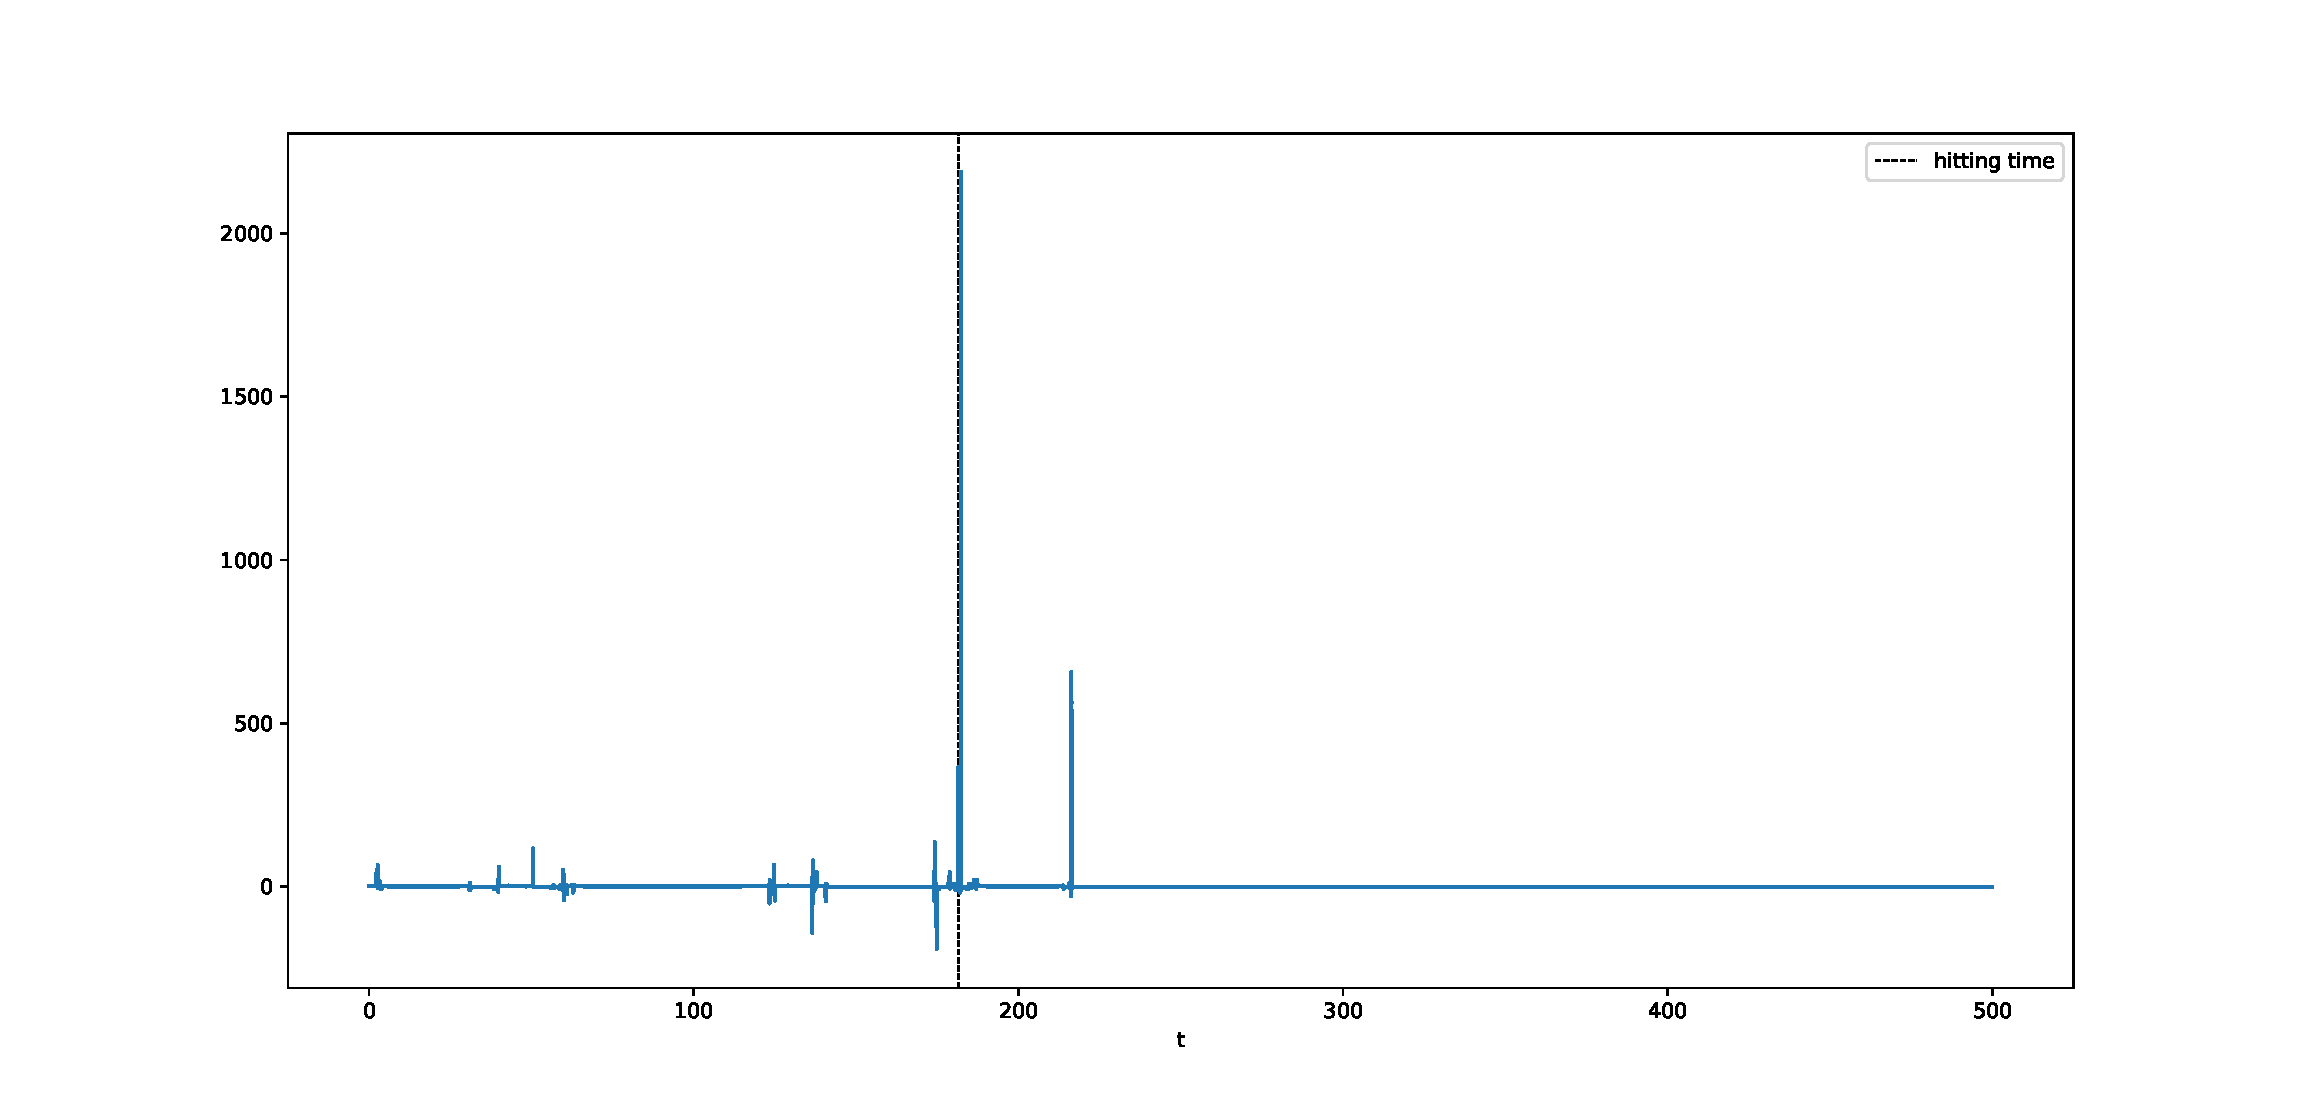
\includegraphics[width=\textwidth]{blowup}
        \caption{Blow-up}
        \label{fig:blowup}
    \end{figure}
    \marginnote{
        It is hard to simulate an exact blow-up (goes to $\infty$)
        and this one is an approximation indeed.
    }

    \problem
    \begin{question}
        The following SDE serves as a counter--example of non-existence of solution after when $W_t$ hits $1$
        \[dX_t=X_t^3dt+X_t^2dW_t, X_0=1.\] 
        i) verify that $X_t=\frac{1}{1-W_t}$ is the solution for $t\in(0,1)$, i.e., it is a solution and it is unique.  Remark: the solution does not exist after $T$, but it exists and is unique before this time;
        
        ii) solve the SDE from scratch paper to get the solution above; hint: try $X_t=f(t,W_t)$; 
        
        iii) test that the solution blow-up by either solving the SDE numerically or plotting the explicit solution above; you might want to record the first time that $W_t$ hits $1$, i.e., the blow-up time; 
        
        iv) note that the time $T$ above is also a random variable now that it depends on the path of $W_t$.  It is called the stopping time as we shall see later in the class.  Can you numerically give an estimate of the mean of $T$?  One way you can do is to, for each trial, record the first time $X_t$ surpass a predetermined large value, say $X_t=10^{16}$.  Then find the average of all the trials;
    \end{question}
    \begin{subproblem}[\roman*)]
        \item
        We have from Taylor's expansion that
        \[\diff X_t=\diff\left(\frac{1}{1-W_t}\right)
        =\frac{\diff W_t}{(1-W_t)^2}
        +\frac{1}{2}\frac{2(\diff W_t)^2}{(1-W_t)^3}
        =X_t^2\diff W_t+X_t^3\diff t\]
        and apparently $X_0=1/(1-W_0)=1$.

        % TODO Prove uniqueness

        \item
        Denote $X_t=f(t,W_t)$, then we have from It\^o's lemma that
        \[\diff X_t=\left(f_t+\frac{f_{xx}}{2}\right)\diff t+f_x\diff W_t\]
        where $f_t$ is short for $\partial f(t,W_t)/\partial t$, $f_{xx}$ for
        $\partial^2 f(t,W_t)/\partial W_t^2$, etc.

        It follows that
        \[f_x=f^2,f_t+\frac{f_{xx}}{2}=f^3\]
        The first equation gives us
        \[f_{xx}=2ff_x=2f^3\]
        Substituting this into the second one gives us
        \[f_t+f^3=f^3\]
        i.e., $f_t=0$.
        Therefore $f_x=f^2$ is an ODE actually, to which the solution is
        \[f(t,W_t)=\frac{1}{C-W_t}\]
        And initial condition $X_0=1$ yields $C=1$, hence
        \begin{equation}
            \label{eq:blow sol}
            X_t=\frac{1}{1-W_t}
        \end{equation}
        With the uniqueness of the SDE, we can conclude that
        the solution is \cref{eq:blow sol}.

        \item
        See \cref{fig:blowup}.

        \item
        We use the average of trials to estimate the expectation.
        After trials of 1000 times with maxtime\marginnote{
            Given an finite time, chances are that the path
            does not hit the line, so we choose the
            hitting time to be assigned to the maxtime.
            And we adjust the maxtime to see the difference
            (the ideal occasion is that the
            maxtime is infinite).

            Actually, we know that the expectation of hitting time of Brownian
            motion is infinite, i.e.,
            \[E(\inf{\{t:W_t=m\}})=\infty,m\in\mathbb R\]
            And we can see that the estimate increases with the maxtime.
        } 1000, 5000, 10000,
        we have an estimate
        of 385.5, 1029.2, 1425.4 accordingly. See \cref{fig:dist}
        for the distributions.
        \begin{figure}[h]
            \centering
            \begin{subfigure}[b]{0.3\textwidth}
                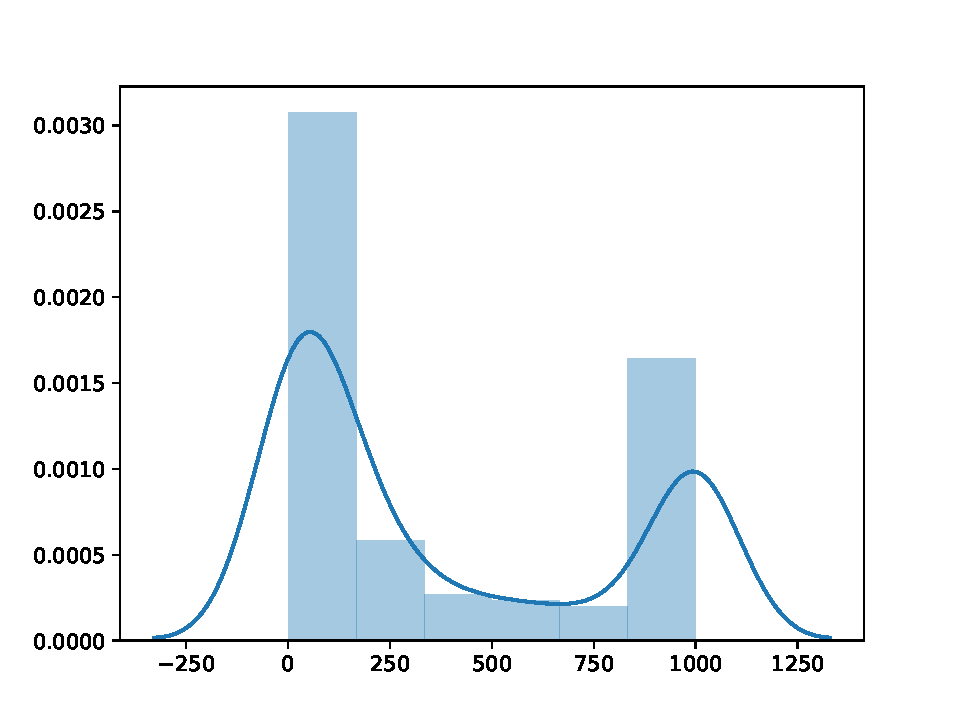
\includegraphics[width=\textwidth]{max=1000}
                \caption{Maxtime 1000}
            \end{subfigure}
            \begin{subfigure}[b]{0.3\textwidth}
                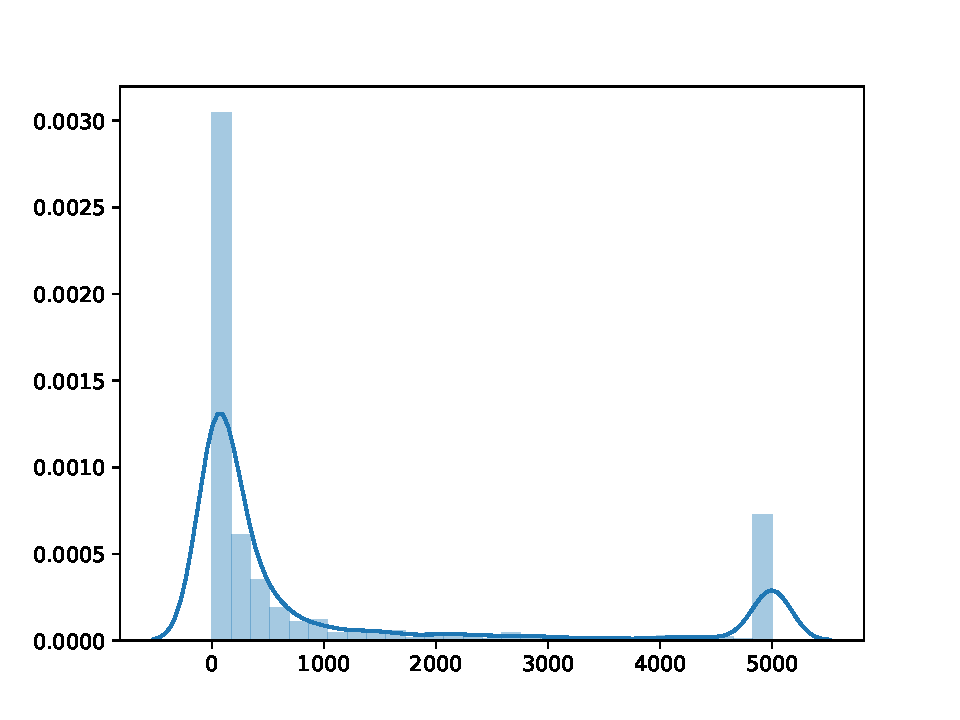
\includegraphics[width=\textwidth]{max=5000}
                \caption{Maxtime 5000}
            \end{subfigure}
            \begin{subfigure}[b]{0.3\textwidth}
                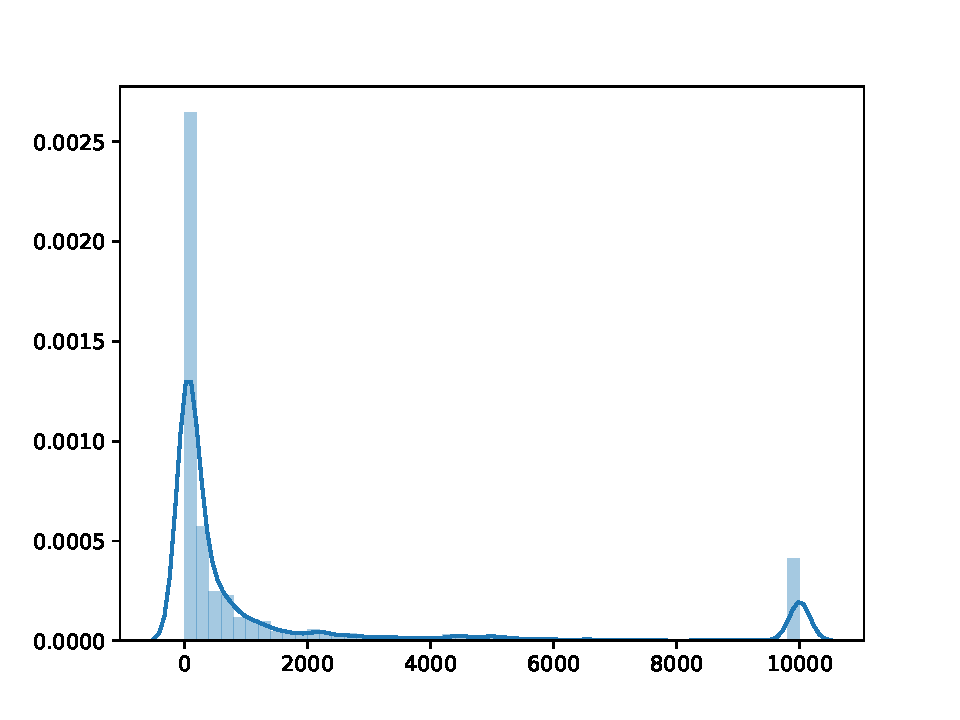
\includegraphics[width=\textwidth]{max=10000}
                \caption{Maxtime 10000}
            \end{subfigure}
            \caption[][3.1cm]{Distribution of hitting time with different maxtime}
            \label{fig:dist}
        \end{figure}
    \end{subproblem}

    \problem
    \begin{question}
        Consider the SDE
        \[dX_t=\Big(\sqrt{1+X^2_t}+\frac{1}{2}X_t\Big)dt+\sqrt{1+X^2_t}dW_t, X_0=x_0.\]
        (a).  Show that there exists a unique solution to this problem;

        (b).  Solve this SDE.
    \end{question}
    \begin{subproblem}
        \item
        \begin{proof}
            Denote $a(t,x)=\sqrt{1+x}+x/2,b(t,x)=\sqrt{1+x^2}$, then
            \[\diff X_t=a(t,X_t)\diff t+b(t,X_t)\diff W_t\]
            And it is easy to see that $a,b$ statisfies Lipschitz condition as
            for any $x,y\in\mathbb R$,
            \[\begin{aligned}
                |a(t,x)-a(t,y)|
                &=\left|\sqrt{1+x^2}-\sqrt{1+y^2}+\frac{x-y}{2}\right|\\
                &\leq\left|\sqrt{1+x^2}-\sqrt{1+y^2}\right|+\frac{1}{2}|x-y|\\
                &=\left(\left|\frac{x+y}{\sqrt{1+x^2}+\sqrt{1+y^2}}\right|+\frac{1}{2}\right)|x-y|\\
                &\leq\left(\left|\frac{x}{\sqrt{1+x^2}}\right|
                +\left|\frac{y}{\sqrt{1+y^2}}\right|+\frac{1}{2}\right)|x-y|\\
                &\leq\frac{5}{2}|x-y|
            \end{aligned}\]
            and similarly
            \[|b(t,x)-b(t,x)|\leq 2|x-y|\]
            We can also verify the sublinear growth condition,
            \[\begin{aligned}
                |a(t,x)|+|b(t,x)|&=\left|\sqrt{1+x^2}+\frac{x}{2}\right|
                +\left|\sqrt{1+x^2}\right|\\
                &\leq 2\left|\sqrt{1+x^2}\right|+\frac{|x|}{2}\\
                &\leq 2(1+|x|)+\frac{|x|}{2}\\
                &\leq \frac{5}{2}(1+|x|)
            \end{aligned}\]
            Then the existence and uniqueness follows as
            as $X_0=x_0$ is a constant.
        \end{proof}

        \item
        Denote\sidenote{The solution is from
        \url{https://math.stackexchange.com/questions/915394/solve-dx-t-sqrt1x-t2-frac12x-t-dt-sqrt1x-t2-dw-t}}
        $\sigma(x):=\sqrt{1+x^2}$, then
        \[\diff X_t=(\sigma(X_t)+X_t/2)\diff t+\sigma(X_t)\diff W_t\]
        And denote $Z_t:=f(X_t)$, where
        \[f(x)=\int_0^x\frac{1}{\sigma(y)}\diff y\]
        then we know that
        \[f'(x)=\frac{1}{\sigma(x)},f''(x)=-\frac{\sigma'(x)}{\sigma^2(x)}\]
        And we have from It\^o's lemma that
        \[\begin{aligned}
            \diff Z_t&=\diff f(X_t)\\
            &=f'(X_t)\diff X_t+\frac{1}{2}f''(X_t)(\diff X_t)^2\\
            &=\left(\frac{f''\sigma^2}{2}
            +\left(\sigma+\frac{X_t}{2}\right)f'\right)\diff t
            +f'\sigma\diff W_t\\
            &=\left(-\frac{\sigma'}{2}+\frac{X_t}{2\sigma}+1\right)\diff t+\diff W_t
        \end{aligned}\]
        where $f$ is short for $f(X_t)$, $\sigma$ for $\sigma(X_t)$ etc.
        But do note that $X_t/\sigma=X_t/\sqrt{1+X_t^2}=\sigma'$, then
        we obtain that
        \[\diff Z_t=\diff t+\diff W_t\]
        which gives us
        \[Z_t=Z_0+t+W_t=f(x_0)+t+W_t\]
        Indeed, one can show that $f(x)=\arcsinh x$
        thus we obtain $X_t$ as
        \[\begin{aligned}
            X_t&=\sinh Z_t\\
            &=\sinh(\arcsinh x_0+t+W_t)\\
            &=x_0\cosh(t+W_t)+\sqrt{1+x_0^2}\sinh(t+W_t)
        \end{aligned}\]
    \end{subproblem}
    
    \problem
    \begin{question}
        Use any method you like to solve \emph{two} of the following SDEs with initial condition $X_0$ for each problem, unless otherwise stated
        \begin{enumerate}[label=(\alph*)]
        \item $dX_t=(4X_t-1)dt+2dW_t$;
        \item $dX_t=(3X_t-2)dt+e^{3t}dW_t$;
        \item $dX_t=(X_t+1)dt+e^t W_t dW_t$;
        \item $dX_t=(4X_t+t)dt+e^{4t}dW_t$;
        \item $t^3 dX_t=(3t^2X_t+t)dt+t^6dW_t$, $X_1=0$;
        \item $dX_t=(\frac{1}{2}X_t+t)dt+e^t \sin W_tdW_t$;
        \item $dX_t=-X_tdt+e^{-t}dW_t$;
        \item $dX_t=X_t^3dt+X_t^2dW_t$, $X_0=1$;
        \item $dX_t=\Big(\sqrt{X^2_t+1}+\frac{1}{2}X_t\Big)dt+\sqrt{X^2_t+1}dW_t$;
        \item $d(\ln r_t)=(\theta(t)-\alpha(t)\ln r_t)dt+\sigma(t)dW_t$;  this is called Black--Karasinki Model
        \end{enumerate}
        Remark: It is strongly recommended that you apply all the methods learnt to work out each problem if applicable, though not required for the HW; moreover, it is also a good practice for you to evaluate the mean and variance with or without solving the SDEs; find the covariance and distribution etc....
    \end{question}
    \begin{subproblem}
        \item[(a)]
        We rewrite the SDE as
        \[\diff X_t-4X_t\diff t=-\diff t+2\diff W_t\]
        and we have from the product rule that
        \[\diff(X_t\e^{-4t})=\e^{-4t}(\diff X_t-4X_t\diff t)\]
        thus
        \[\diff(X_t\e^{-4t})=-\e^{-4t}\diff t+2\e^{-4t}\diff W_t\]
        which gives us
        \[X_t\e^{-4t}-X_0=\frac{\e^{-4t}-1}{4}+2\int_0^t\e^{-4s}\diff W_s\]
        And we also have from integration by parts that
        \[\int_0^t\e^{-4s}\diff W_s=W_s\e^{-4s}|_0^t+4\int_0^tW_s\e^{-4s}\diff s
        =W_t\e^{-4t}+4\int_0^tW_s\e^{-4s}\diff s\]
        Finally we obtain $X_t$ as
        \[X_t=\frac{1}{4}+\left(X_0-\frac{1}{4}\right)\e^{4t}+2W_t+8\int_0^tW_s\e^{-4s}\diff s\]

        \item[(e)]
        We rewrite the SDE as (assume that $t>0$)
        \[\diff X_t-\frac{3}{t}X_t\diff t=\frac{\diff t}{t^2}+t^3\diff W_t\]
        and we have from the product rule that
        \[\diff\left(\frac{X_t}{t^3}\right)=t^{-3}\diff X_t+X_t\diff(t^{-3})
        =t^{-3}\left(\diff X_t-\frac{3}{t}X_t\diff t\right)\]
        It follows that
        \[\diff\left(\frac{X_t}{t^3}\right)=\frac{\diff t}{t^5}+\diff W_t\]
        which gives us
        \[\frac{X_t}{t^3}-X_1=\int_1^t\frac{1}{s^5}\diff s+W_t-W_1
        =\frac{1}{4}\left(1-\frac{1}{t^4}\right)+W_t-W_1\]
        Therefore,
        \[X_t=\frac{1}{4}\left(t^3-\frac{1}{t}\right)+t^3(W_t-W_1)\]
        as $X_1=0$.
    \end{subproblem}

    \appendix
    \section{Python Code}
    \lstinputlisting[language=Python]{blowup.py}
